
\begin{enumerate}
    \item que es la luminiscencia? algunas aplicaciones ej. microscopía, plim y flim
    \begin{itemize}
        \item In 1565, a Spanish physician and botanist, Nicolas Monardes (Figure 2), reported the peculiar blue color (under certain  conditions of observation) from an infusion of a wood from Mexico and used to treat kidney and urinary diseases (Figure 3). 912 This wood (later called Lignum nephriticum), whose peculiar color effect and diuretic properties were already known to the Aztecs, was a scarce and expensive medicine. Therefore, it was of interest to detect counterfeited wood. Monardes wrote on this respect, 12 Make sure that the wood renders water bluish, otherwise it is a falsification. Indeed, they now bring another kind of wood that renders the water yellow, but it is not good, only the kind that renders the water bluish is genuine. (in Spanish in the original). This method for the detection of a counterfeited object can be considered as the first application of the phenomenon that would be later called fluorescence. Extracts of the wood were further investigated by Boyle, Newton, and others, 6 but the phenomen- on was not understood at the time.
        \item n 1845, the polymath Sir John Herschel, son of the famous astronomer and the originator of the word photography (where light is again involved), prepared an acid solution of quinine sulfate and stated,18 Though perfectly transparent and colorless when held between the eye and the light, it yet exhibits in certain aspects, and under certain incidences of the light, an extremely vivid and beautiful celestial blue color. As the color was always superficial, he believed it to be a hitherto unidentified phenomenon, “a case of superficial colour presented by a homogeneous liquid, internally colourless”. 18 Herschel called this phenomenon epipolic dispersion, from the Greek: επιπολη = surface. In fact, the solutions observed by Herschel were very concentrated so that the majority of the incident light was absorbed near the surface and all the blue fluorescence originated from there. Herschel used a prism to show that the epipolic dispersion could be observed only upon illumination by the blue end of the spectrum and not the red end. The crude spectral analysis of the emitted light with the prism revealed blue, green, and a small quantity of yellow light, but Herschel did not realize that the superficial light was of longer wavelength than the incident light.
        \item One of Stokes’s experiments that is spectacular and remarkable by its simplicity deserves attention. Stokes formed the solar spectrum by means of a prism. When he moved a test tube filled with a solution of quinine through the visible part of the spectrum, nothing happened: the solution remained transparent. 20 But beyond the violet portion of the spectrum, that is, in the invisible zone corresponding to ultraviolet radiation, the solution glowed with a blue light (Figure 7). Stokes wrote, 4 It was certainly a curious sight to see the tube instantaneously light up when plunged into the invisible rays: it was literally darkness visible. Altogether the phenomenon had something of an unearthly appearance. From his experiments with a wide range of substances, Stokes concluded that the dispersed light was always of longer wave- lengths than the incident light. Later this statement became the Stokes law. Stokes also noted that the dispersion of light took place in all directions, hence, the fluid behaved as if it were self-luminous. In his paper, Stokes called the observed phenomenon true internal dispersion or dispersive reflection but in a footnote, 4 he wrote, I confess I do not like this term. I am almost inclined to coin a word, and call the appearance fluorescence, from fluorspar, as the analogous term opalescence is derived from the name of a mineral. In his second paper, 21 Stokes definitely resolved to use the word fluorescence.
        \item Luminescence is an emission of ultraviolet, visible or infrared photons from an electronically excited species. The word luminescence, which comes from the Latin (lumen ¼ light) was first introduced as luminescenz by the physicist and science historian Eilhardt Wiedemann in 1888, to describe ‘all those phenomena of light which are not solely conditioned by the rise in temperature’, as opposed to incan- descence. Luminescence is cold light whereas incandescence is hot light. The various types of luminescence are classified according to the mode of excitation (see Table 1.1).
        \item The success of fluorescence as an investigative tool in studying the structure and dynamics of matter or living systems arises from the high sensitivity of fluoro- metric techniques, the specificity of fluorescence characteristics due to the micro- environment of the emitting molecule, and the ability of the latter to provide spatial and temporal information. Figure 1.3 shows the physical and chemical parameters that characterize the microenvironment and can thus affect the fluorescence char- acteristics of a molecule.
        \item As a consequence of the strong influence of the surrounding medium on fluores- cence emission, fluorescent molecules are currently used as probes for the investi- gation of physicochemical, biochemical and biological systems. A large part of this book is devoted to the use of so-called fluorescent probes.
        \item An electronic transition consists of the promotion of an electron from an orbital of a molecule in the ground state to an unoccupied orbital by absorption of a photon. The molecule is then said to be in an excited state. Let us recall first the various types of molecular orbitals.
        \item Additionally, fluorescence is used for cell identification and sorting in flow cytometry, and in cellular imaging to reveal the localization and movement of intracellular substances by means of fluores- cence microscopy.
        \item It is interesting to notice that the first known fluoro- phore, quinine, was responsible for stimulating the devel- opment of the first spectrofluorometers, which appeared in the 1950s. During World War II, the Department of De- fense was interested in monitoring antimalaria drugs, in- cluding quinine. This early drug assay resulted in a subsequent program at the National Institutes of Health to develop the first practical spectrofluorometer.*
    \end{itemize}
    \item hamiltoniano de un átomo de muchos electrones? - si hago esto, el foco debería ser \\
    por qué las cosas emiten o no emiten?
    \item diagrama de jablonski. Cómo se convierte la excitación del electrón en luz? \\
    de qué otras formas puede convertirse la energía del electrón?
    decaimientos radiativos y no radiativos. \\
    ver seccion jablonski del lakowicz
    \item fluorescencia y fosforescencia diferencias -> transiciones prohibidas y tiempos de vida
    \item corrimiento stokes y anti stokes -> fenómenos de muchos fotones
    \item caracterización de luminiscencia estática
    \item caracterización de luminiscencia dinámica -> TCSPC
    \item Nanopartículas de upconversion, composición y aplicaciones
    \item fotofísica de los lantánidos
    \item mecanismos principales de upconversión
    \item dependencia con la potencia de excitación
    \item modelos de la dinámica de las nanopartículas
    \item que hace falta para caracterizar las nanopartículas?
\end{enumerate}


\newpage


En 1565, el médico y botanista Nicolás Monardes reportó el peculiar color azul que tomaba una infusión de madera mexicana usada para tratar enfermedades de riñón y urinarias. Este efecto ya era conocido por los Aztecas, que lo utilizaban para asegurarse que la valiosa madera no fuera falsificada. Monardes escribe en su libro \cite{valeur_introduction_2012}

\begin{quote}
    \textit{Asegúrate de que la madera torne el agua azulada, de lo contrario, es una falsificación. De hecho, ahora traen otro tipo de madera que torna el agua amarilla, pero no sirve; solo el tipo que torna el agua azulada es genuina.}
\end{quote}  

\noindent Años más tarde, en 1845, el matemático Sir John Herschel describió el efecto similar que producía una solución transparente de quinina, una sustancia presente en el agua tónica, que reflejaba \flqq un color azul celestial hermoso y extremadamente vívido\frqq.
Herschel usó un prisma para comprobar que la dispersión causada por la quinina sólo se observaba al iluminar la solución con la parte azul del espectro.
El mismo análisis para la luz emitida reveló luz azul, verde, y una pequeña cantidad de amarillo.
En esa misma época, el físico Sir George Gabriel Stokes publicó \textit{On the Refrangibility of Light}, un trabajo explicando experimentos con múltiples sustancias que exhibían este tipo de comportamientos, entre ellas incluida la quinina.
Uno de sus experimentos más importantes consistía en formar el espectro solar a partir de un prisma, para luego mover un tubo de ensayo con la solución de quinina a través de sus colores.
La solución permanecía transparente al ser iluminada por la parte visible del espectro, pero al llegar a la zona ultravioleta (invisible al ojo humano), la muestra se iluminó con luz azul brillante.
Además de concluir que la luz siempre se dispersaba con longitudes de onda mayores a las de incidencia, afirmación que luego se conocería como corrimiento de Stokes, llamó a este fenómeno \textit{fluorescencia} \cite{valeur_introduction_2012}.

En 1888, el físico Eilhardt Wiedmann introdujo el término luminiscencia para referirse a los fenómenos lumínicos que no están determinados por un aumento en la temperatura de los materiales.
Entre ellos estan la fosforescencia y la fluorescencia.
Actualmente ambos tienen aplicaciones en múltiples areas distintas del conocimiento y la tecnología. 
Es particularmente destacable su éxito como herramienta para estudiar la estructura y dinámica de la materia viva, gracias la sensibilidad al micro-entorno de las moléculas fluorescentes, lo que resulta en una alta resolución espacial y temporal. 
Por ejemplo, la microscopía de fluorescencia consiste en iluminar la muestra con una longitud de onda y detectar su fluorescencia en otra, permitiendo filtrar el fondo de la imagen \cite{valeur_introduction_2012}.
Técnicas dinámicas como la microscopía de imágenes de tiempo de vida de fluorescencia (FLIM) o fosforescencia (PLIM) dan lugar a conocer el entorno químico en el que se encuentran distintas proteinas, como su PH, viscosidad, temperatura, entre otras cantidades \cite{suhling_fluorescence_2015} \cite{baggaley_timeresolved_2015}.
Si bien en el siglo 19 ya se sabía que los mecanismos de emisión de luz de estos fenómenos no estaban vinculados al aumento de temperatura de los materiales, no fue hasta el desarrollo de la mecánica cuántica a principos del 20 que se entendió su causa: la luminiscencia está dada por la transición entre distintos estados de energía de los electrones.

\section{Luminiscencia}


\begin{figure}
    \centering
    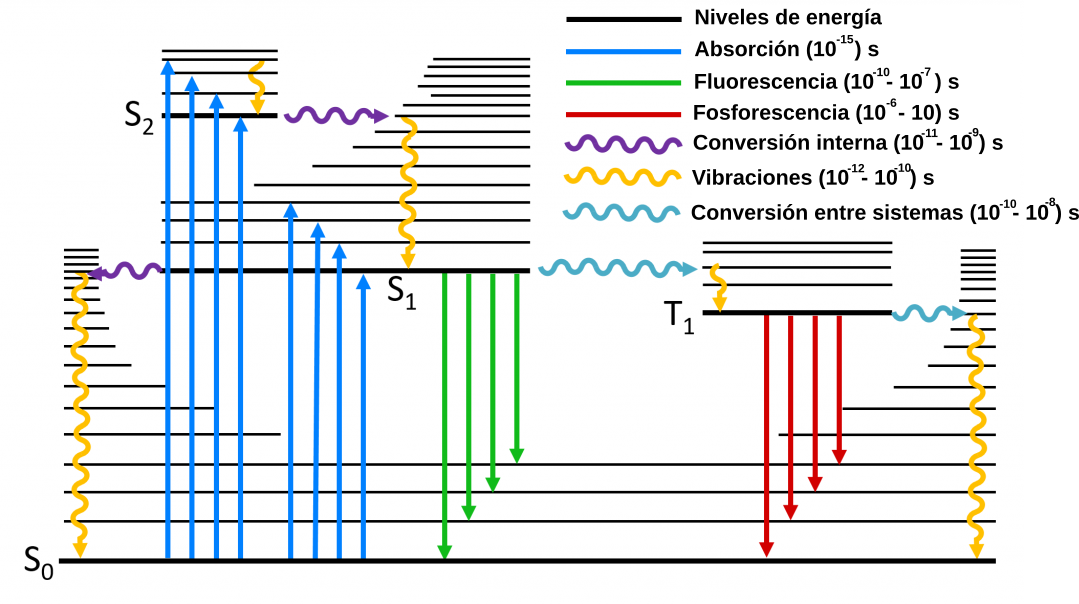
\includegraphics[width=\textwidth]{jablonski}
    \caption{\textbf{Diagrama de Jablonski.}}
    \label{fig:jablonski}
\end{figure}

\subsection{Espectroscopía estática}

La luminiscencia es la emisión de fotones mediante la transición de un electron en un estado excitado con energía $E_e$ a otro con energía $E_k < E_e$.
Este proceso suele ilustrarse a través de un diagrama de Jablonski (\textbf{Fig. \ref{fig:jablonski}})\footnote{Tomado de \href{https://edinst.com/wp-content/uploads/2019/02/JablonskiDiagramFull-1024x604.png}{https://edinst.com/wp-content/uploads/2019/02/JablonskiDiagramFull-1024x604.png}}.
En un diagama de Jablonski se muestran los niveles de energía electrónicos del material luminiscente junto con las posibles transiciones entre ellos.
En el diagrama se ven los estados singlete $S_0$, $S_1$ y $S_2$, y el estado triplete $T_1$.
Todo proceso luminiscente comienza con la absorción de un fotón, lo que lleva al electrón a un estado más energético.
Estas absorciones ocurren en un lapso de $10^{-15}$ s, un tiempo suficientemente corto como para que los desplazamientos de los núcleos del sistema sean despreciables \cite{lakowicz_principles_2006}.
La diferencia de energía entre estos estados es típicamente del orden de los eV.
A su vez, un electrón en un dado estado electrónico puede estar en distintos estados vibracionales, aunque estos estados estan separados por energías del orden de las décimas de eV.
Las transiciones entre estados vibracionales también son posibles y ocurren en un lapso de $10^{-12}$ a $10^{-10}$ segundos.

La sucesión de este tipo de transiciones da lugar a la fluorescencia: un electrón absobe un fotón altamente energético, excitándolo a un estado electrónico de mayor energía con vibraciones.
Rápidamente sus oscilaciones se relajan, dejándolo en un estado electrónico excitado, pero con baja energía vibracional.
Por último, el electrón vuelve a su estado fundamental re-emitiendo un fotón, pero esta vez de menor energía que el que había absorbido.
La fluorescencia tiene tiempos típicos de $10^{-10}$ a $10^{-7}$ segundos.
El método más usual para caracterizar un material fluorescente, o luminiscente en general, es a través de su espectro de emisión y de absorción.
Alternativamente, uno puede medir el espectro de excitación, que está fuertemente relacionado con el de absorción.
El proceso para medir cada uno es:

\begin{itemize}
    \item \textbf{Emisión:} consiste en medir la intensidad de luz emitida por la muestra en un rango amplio de longitudes de onda $\Delta \lambda_{em}$, al ser excitada por una longitud de onda fija $\lambda_{ex}$.
    \item \textbf{Absorción:} requiere medir la intensidad de luz que absorbe la muestra. Esto generalmente se logra excitando una solución de la sustancia en un rango de longitudes de onda y midiendo la cantidad de luz transmitida en cada caso.
    \item \textbf{Excitación:} para obtener este espectro se debe medir la intensidad de luz emitida por la muestra una dada longitud de onda $\lambda_{em}$, y barrer la excitación en un rango $\Delta \lambda_{ex}$.
\end{itemize}

\noindent La figura (\textbf{\ref{fig:fluoresceina}}) muestra el espectro de absorción y de emisión de la fluoresceina, una tinta orgánica utilizada en distintas técnicas de diagnóstico médico \cite{fluoresceina_1,fluoresceina_2}.
Los espectros dejan en evidencia la fluorescencia de la molécula: absorbe fotones de $457$ y $486$ nm, es decir $2.71$ eV y $2.55$ eV respectivamente, y emite con mayor intensidad en $523$ nm, equivalente a $2.37$ eV.
Previsiblemente, la diferencia de energía es de $\sim 0.2$ eV, en el rango de energías vibracionales.


\begin{SCfigure}
    \centering
    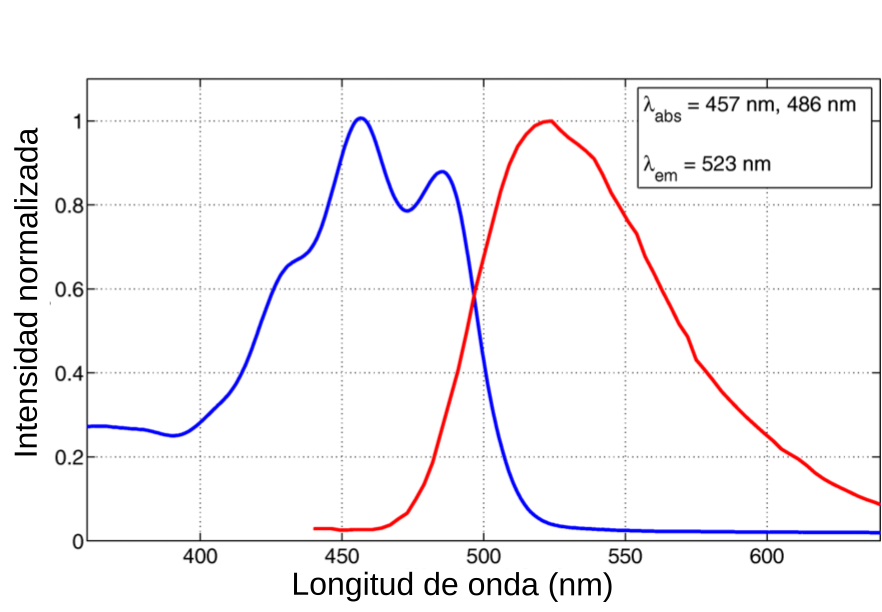
\includegraphics[width=0.7\textwidth]{fluoresceina_espectro.png}
    \caption{\textbf{Espectro de la Fluoresceina} diluida en etanol, tanto de absorción (azul) como de emisión (rojo). El cuadro muestra los picos de absorción en $\lambda_{abs}=457$ nm y 486 nm, y de emisión en $\lambda_{em}$ = 523 nm. Tomada y adaptada de \cite{kristoffersen_testing_2018}.}
    \label{fig:fluoresceina}
\end{SCfigure}

Otro tipo de mecanismos presentes en los materiaes luminiscentes son la conversión interna y la conversión entre sistemas.
Ambos consisten en transiciones entre estados electrónicos excitados, el primero es entre estados de la misma multiplicidad, en general singlete-singlete, y el segundo se da entre estados singlete-triplete \cite{valeur_characteristics_2012}.
La conversión entre sistemas, que ocurre en el orden de $10^{-10}$ a $10^{-9}$ segundos, es la responsable de la fosforescencia.
La fosforescencia es la transición de un electrón en un estado excitado triplete a un estado singlete de menor energía.
A diferencia de las transiciones fluorescentes, las transiciones triplete-singlete estan prohibidas por las reglas de selección de la mecánica cuántica \cite{demtroder_emission_2010}.
Por este motivo, los tiempos característicos de la fosforescencia son mucho mayores, del orden de $10^{-6}$ hasta $10$ segundos.
Además de los espectros de absorción, emisión y excitación, los tiempos de estas transiciones son de gran relevancia para caracterizar a los materiales luminiscentes.

\subsection{Espectroscopía dinámica}

\begin{SCfigure}
    \centering
    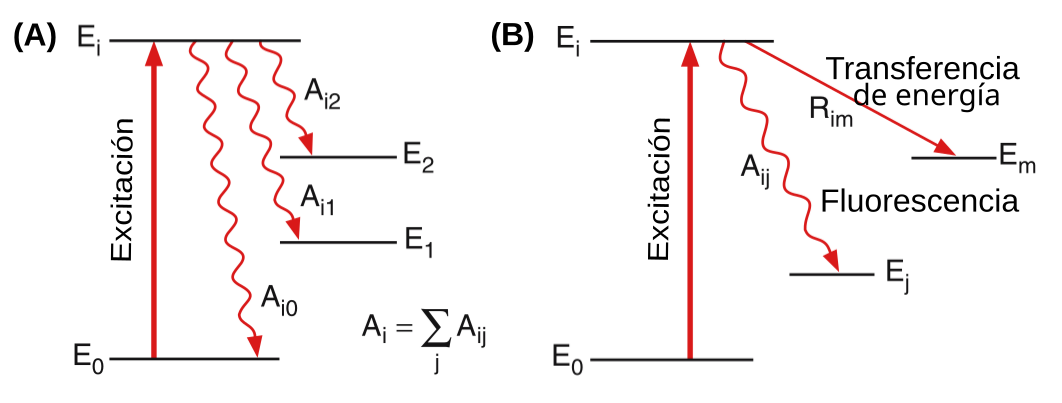
\includegraphics[width=0.7\textwidth]{transiciones_tiempo.png}
    \caption{\textbf{Diagrama de Jablonski} con transiciones que contribuyen al tiempo de vida.\textbf{(A)} Sólo transiciones de fluorescencia. \textbf{(B)} Transiciones de fluorescencia y choques. Tomado y adaptado de \cite{demtroder_emission_2010}.}
    \label{fig:transiciones_tiempo}
\end{SCfigure}


Se le llama tiempo de vida medio al tiempo promedio que el electrón pasa en un estado excitado de energía.
La caracterización del tiempo de vida medio no solo brinda información del elemento luminiscente, sino también de su entorno.
Es necesario hablar de tiempos medios porque las transiciones son un fenómeno fundamentalmente cuántico, y por lo tanto un proceso aleatorio.
Además, la mayoría de mediciones de luminiscencia se hacen con una muestra que presenta grandes cantidades de los elementos ópticamente activos, por lo que también hay un efecto aleatorio propio de esa estadística.

Si se tienen $N_i$ átomos en un estado excitado con energía $E_i$ y se asume que la probabilidad de transición a un estado de menor energía $E_j$ es constante en el tiempo se obtiene que

\begin{equation} \label{eq:lifetime}
    \frac{dN_i}{dt} = A_{ij} N_i \implies N_i(t) = N_i(0)e^{A_i t},
\end{equation}

\noindent donde $A_{ij}$ es una constante llamada coeficiente de Einstein, y $A_i = \sum_{j} A_{ij}$ tiene en cuenta la probabilidad de el electrón decaiga a cualquier estado con $E_j < E_i$ (ver \textbf{Fig. \ref{fig:transiciones_tiempo}A}) \cite{demtroder_emission_2010}.
Como sabemos que un electrón emite un fotón al desexcitarse, la ecuación (\ref{eq:lifetime}) nos dice que al dejar de iluminar una muestra esperamos que se emitan fotones exponencialmente distribuidos en el tiempo.
Es decir que si tenemos un detector de fotones, medimos con precisión el tiempo en el que dejamos de iluminar, y hacemos un histograma de los tiempos en los que detectamos un fotón, las alturas de sus barras deberían seguir una exponencial.
Además sabemos que la relación entre el tiempo de vida y el parámetro de la exponencial es $\tau_i = 1/A_i$, por lo que es posible ajustar una exponencial a la altura de las barras para medirlo.
Exactamente eso es lo que se hace en \textit{Time-Correlated Single Photon Counting} (TCSPC, ver sección \ref{sec:intro_tcspc}), una de las técnicas más comunes para medir tiempos de vida.

La ecuación (\ref{eq:lifetime}) sólo tiene en cuenta las transiciones fluorescentes del átomo, pero como explicamos en la sección anterior, éstas no son las únicas.
Además, generalmente los átomos estan en entornos que inducen transiciones no radiativas, como transferencia de energía a otros átomos, o colisiones con átomos vecinos (\textbf{Fig. \ref{fig:transiciones_tiempo}B}). 
Suponiendo que se induce una nueva probabilidad de desexcitación no radiativa $R_i$ por transferencia de energía, y siguiendo la lógica anterior, la tasa de cambio de cantidad de átomos $N_i$ en el estado $i$ es

\begin{equation}
    \frac{dN_i}{dt} = (A_{ij} + R_i) N_i \implies N_i(t) = N_i(0)e^{(A_i + R_i) t},
\end{equation}

\noindent y por lo tanto su tiempo de vida efectivo $\tau_{eff} = 1/(A_i + R_i)$. 
La implicancia de este fenómeno es muy fuerte: es posible obtener información del entorno microscópico de un material luminiscente al medir su tiempo de vida \cite{ryder_timedomain_2001}.

Para poder aprovechar estas propiedades de los materiales luminiscentes es necesario poder medir precisamente tanto sus espectros estacionarios como los dinámicos. 
En la próxima sección comentamos brevemente cuáles son los instrumentos y técnicas que se implementan más comunmente para hacer este tipo de mediciones.


\section{Instrumentación para espectrometría de fluorescencia}

\subsection{El espectrofluorímetro}

Para caracterizar la respuesta óptica de una sustancia, generalmente se desea registrar tanto el espectro de excitación como el de emisión. 
El instrumento científico por excelencia para realizar estas mediciones es el espectrofluorímetro. 
Fundamentalmente, este instrumento permite realizar mediciones de la intensidad de luz que emite una muestra, haciendo escaneos en longitud de onda de emisión y excitación.
Adicionalmente, algunos pueden realizar mediciones de tiempo de vida resueltas, escaneos sincrónicos con alguna señal y mediciones de anisotropía en la polarización de materiales luminiscentes.
Estas capacidades son fundamentales para investigaciones en diversas disciplinas científicas, incluyendo química, bioquímica, farmacología, ciencias ambientales, ciencia de materiales y biomedicina.
El objetivo principal de un espectrofluorímetro es obtener los espectros de emisión y de excitación de una muestra.
Para lograr este objetivo, el instrumento debe ser capaz de iluminar la muestra con múltiples longitudes de onda diferentes y registrar su respuesta a cada una de ellas.

La Figura 2.1 muestra un diagrama esquemático de un espectrofluorímetro genérico.
Este instrumento incluye todos los componentes fundamentales para cumplir su función. 
Utiliza una lámpara de espectro amplio que funciona como fuente de luz de alta intensidad para un rango extenso de longitudes de onda. 
Posteriormente la luz es filtrada por un monocromador de excitación que permite seleccionar la longitud de onda con la que se desea iluminar a la muestra.
La luz de excitación seleccionada se enfoca sobre la muestra colocada en la cámara principal, cuya luminiscencia, generalmente con una longitud de onda mayor que la luz de excitación, es filtrada por el monocromador de emisión.
Los monocromadores suelen estar motorizados, lo que permite que el escaneo sea automático. 
La luz restante llega a un detector, usualmente un tubo fotomultiplicador (PMT), un detector muy sensible que convierte fotones en corriente eléctrica.
El espectrofluorímetro emplea diversas técnicas para reducir la luz parásita (longitudes de onda diferentes a la deseada), como el diseño en ángulo de 90° entre los brazos de excitación y emisión, y un compartimento hermético pintado de negro no reflectante.
La señal del PMT es procesada electrónicamente, digitalizada y analizada en una computadora. 
Este sistema también controla los monocromadores y la adquisición de datos, además de permitir al usuario ajustar parámetros y facilitar la visualización y análisis.
A menudo, se incorporan componentes adicionales en el camino óptico, como obturadores, polarizadores, divisores de haz y otros elementos ópticos, para estudiar diferentes propiedades de la muestra.

\begin{SCfigure}
     \centering
     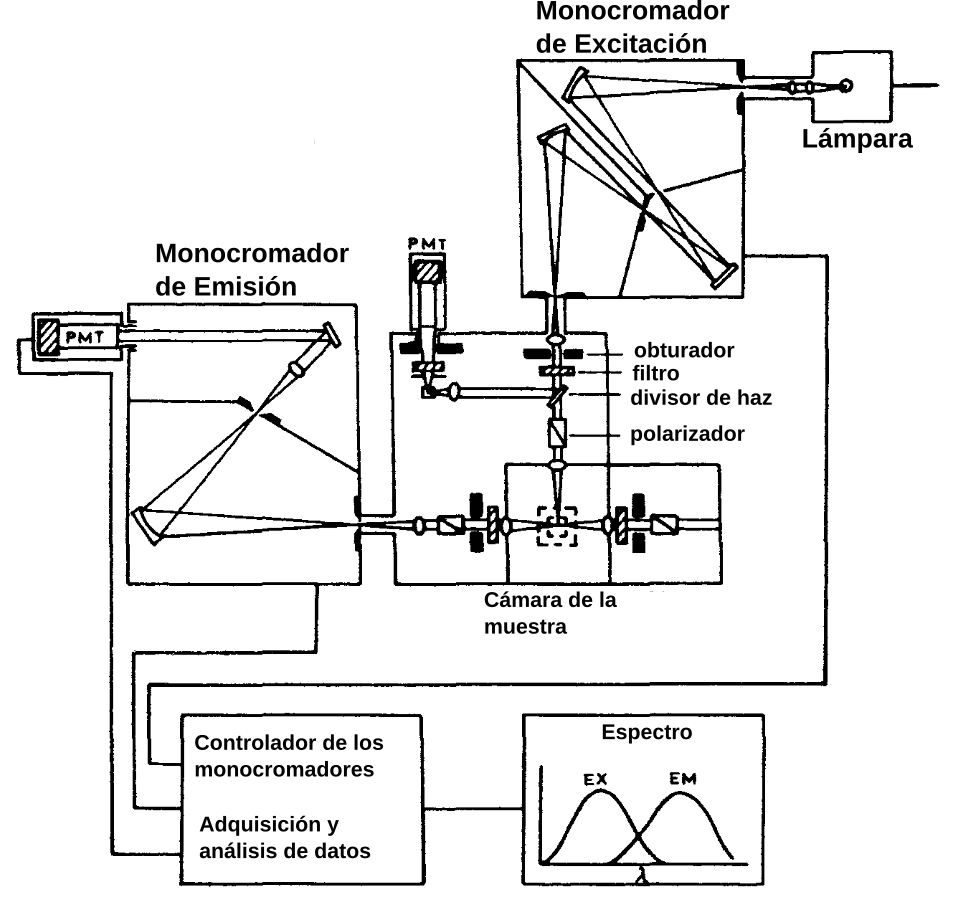
\includegraphics[width=0.6\textwidth]{spectrometer_diagram_lako_modif.png}
     \caption{
    \textbf{Diagrama de un espectrofluorímetro genérico.}
    La luz traza un camino que comienza en la lámpara (zona superior derecha) y termina en el PMT de detección (centro izquierda). Después de salir de la lámpara, la luz es filtrada por un monocromador y luego enfocada sobre la muestra. La luz reemitida pasa por otro monocromador y termina en el PMT. La señal se lee con un sistema de control que la digitaliza y para luego ser procesada por una PC que construye los espectros. Figura tomada y adaptada de \cite{lakowicz_principles_2006}.
    }
     \label{fig:spec_diagram_lako}
\end{SCfigure}


\todo{el mio es el mas comun pero no es el único que existe}

\subsection{Epectrofluirimetros en argentina y obsolescencia}

Actualmente, el Departamento de Física de la FCEyN-UBA no cuenta con espectrofluorímetros para la caracterización de espectros de excitación y emisión.  
Para realizar este tipo de mediciones, la facultad dispone del laboratorio de fotoquímica del Instituto de Química Física de los Materiales, Medio Ambiente y Energía (INQUIMAE), que cuenta con tres espectrofluorímetros con distintas características, pero que tienen algo en común: ningún equipo tiene menos de 20 años, el más antigüo llegando a los 40 años de uso.
La disparidad en al antigüedad y funcionalidad de los instrumentos es un fenómeno común en laboratorios de investigación en países como Argentina, donde la inversión en ciencia es escasa o poco regular en el tiempo \cite{cioccaRealityScientificResearch2017}. 
Ante esta realidad, los institutos suelen priorizar la adquisición de equipos con nuevas capacidades, en lugar de renovar instrumentos existentes por versiones más modernas.  
Esto es posible gracias a la precisión y robustez de las partes mecánicas de los instrumentos, pero la obsolescencia de los equipos antiguos plantea problemas a largo plazo, especialmente cuando sus plataformas de control quedan desactualizadas.  
Con el tiempo, se vuelve complicado operar estos instrumentos, ya que los mecanismos de extracción de datos, como los disquetes, dejan de estar disponibles en el mercado. 
Aún más crítico es que el funcionamiento del equipo depende de la computadora de control, la cual utiliza placas y puertos que ya no se fabrican ni se consiguen en el mercado actual.  
El problema de la obsolescencia en instrumentos científicos afecta desproporcionadamente a instituciones con bajo presupuesto, ampliando la brecha de accesso a instrumentos de investigación avanzados.

Esto ha llevado a un auge en el desarrollo de instrumentos científicos accesibles y de bajo costo \cite{wenzel_open_2023, arancio_inequalities_2023}, particularmente en áreas como instrumentación, microscopía, espectroscopía y adquisición de datos \cite{jameson_fluorescent_1989, li_optical_2022, hu_fluorescent_2022}.
Las iniciativas de hardware abierto hacen que los diseños y la documentación estén disponibles de forma gratuita para que cualquier persona pueda usarlos, construirlos y modificarlos \cite{powell_democratizing_2012, oellermann_open_2022}.
Por ejemplo, la plataforma Arduino ha proporcionado una plataforma de desarrollo de electrónica económica y fácil de usar basada en un microcontrolador (https://www.arduino.cc/).
El OpenFlexure Microscope es un microscopio de código abierto que cuesta menos de 100 USD construir \cite{collins_robotic_2020}.
Asimismo, recientemente se desarrolló un espectrómetro basado en Raspberry Pi que cuesta menos de 400 EUR \cite{tunens_optical_2024}.
El software y los lenguajes de código abierto, como Python (http://www.python.org), que cuentan con bibliotecas numéricas y de instrumentación como NumPy \cite{harris_array_2020} y PyVISA \cite{grecco_pyvisa_2023}, han desempeñado un papel clave al reducir las barreras de entrada y facilitar la creación rápida de prototipos.
Cabe destacar que han surgido empresas enfocadas en hardware parcialmente o completamente abierto. Por ejemplo, OpenBCI (https://openbci.com/), que ofrece sistemas EEG de bajo costo para interfaces cerebro-computadora, y Opentrons (https://opentrons.com/), que proporciona soluciones de manejo de líquidos para la automatización de laboratorios.


\section{Espectrofotometría estática}
\section{Espectrofotometría dinámica} 

\subsection{Medición de tiempos de vida: \textit{Time-Correlated Single Photon Counting}} \label{sec:intro_tcspc}

Muchos espectrofluorímetros comerciales tienen la capacidad de medir el tiempo de vida de los fluoróforos con tiempos típicos del orden de los nanosegundos. 
Sin embargo, debido a las transiciones prohibidas de los lantánidos (\todo{Ver cap N}) el tiempo de vida de las UCNPs es del orden de los cientos de microsegundos.
Aunque esto alivia la necesidad de una electrónica rápida y costosa, contradictoriamente hace que no se pueda medir su tiempo de vida en instrumentos comerciales, ya que los valores típicos están muy alejados del rango en el que operan \cite{bujjamer2020}.

Existen distintas técnicas para medir el tiempo de vida \cite{becker_fluorescence_2012}, pero la más implementada es \textit{Time-Correlated Single Photon Counting} (TCSPC).
Como la técnica se suele aplicar para tiempos de vida del orden de los nanosegundos es común que se usen componentes de electrónica rápida 
Usualmente la explicación de esta técnica involucra introducir múltiples componentes de electrónica rápida que son necesarios para medir tiempos del orden de nanosegundos.
Como en nuestro caso esos componentes no son necesarios, daremos una explicación simplificada.
TCSPC es una técnica digital que cuenta fotones correlacionados temporalmente con respecto a un pulso de excitación.
El experimento comienza con un pulso de excitación, que tiene dos tareas fundamentales: (i) excitar a la muestra y (ii) iniciar algún tipo de cronómetro.
La muestra se excita repetidamente utilizando una fuente de luz pulsada, a menudo un láser o una lámpara de destellos.
Cada pulso es monitoreado, produciendo una señal de inicio que activa el contador del cronómetro.
La rampa de voltaje se detiene cuando se detecta el primer fotón de fluorescencia proveniente de la muestra.
El TAC proporciona un pulso de salida cuyo voltaje es proporcional al tiempo transcurrido entre las señales de inicio y parada.
Un analizador multicanal (MCA) convierte este voltaje en un canal de tiempo utilizando un convertidor analógico a digital (ADC).
Sumando sobre muchos pulsos, el MCA genera un histograma de probabilidad de cuentas frente a los canales de tiempo.

\section{Nanopartículas de conversión ascendente} \label{sec:intro_ucnp}